\documentclass[letterpaper,10pt,onecolumn]{article}
\usepackage[spanish]{babel}
\usepackage[latin1]{inputenc}
\usepackage{amsfonts}
\usepackage{amsthm}
\usepackage{amsmath}
\usepackage{mathrsfs}
\usepackage{empheq}
\usepackage{enumitem}
\usepackage[pdftex]{color,graphicx}
\usepackage{hyperref}
\usepackage{listings}
\usepackage{calligra}
\usepackage{algpseudocode} 
\DeclareMathAlphabet{\mathcalligra}{T1}{calligra}{m}{n}
\DeclareFontShape{T1}{calligra}{m}{n}{<->s*[2.2]callig15}{}
\newcommand{\scripty}[1]{\ensuremath{\mathcalligra{#1}}}
\lstloadlanguages{[5.2]Mathematica}
\setlength{\oddsidemargin}{0cm}
\setlength{\textwidth}{490pt}
\setlength{\textheight}{610pt}
\setlength{\topmargin}{-85pt}
\addtolength{\hoffset}{-0.3cm}
\addtolength{\textheight}{4cm}

\begin{document}
\thispagestyle{empty}
\begin{center}


\includegraphics[width=490pt]{figs/header.png}\\[0.5cm]

\textsc{\LARGE Parcial 1 - F\'isica I (FISI-1018) - 2016-10}\\[0.5cm]

\textsc{\Large{Profesor: Jaime Forero --- Fecha: Febrero 16, 2016}} \\[0.5cm]
\end{center}

Yo, \rule{10cm}{0.4pt}, con c\'odigo \rule{4cm}{0.4pt} de Uniandes,
acepto hacer este ex\'amen sin ayuda ni copia de fuentes no
permitidas (incluyendo libros, notas y cualquier dispositivo
electr\'onico),  sabiendo que hacer lo contrario va a ser considerado
como fraude (una falta grave que se sanciona hasta con suspenci\'on de la Universidad por
dos semestres como consta en el cap\'itulo X del reglamento general de
estudiantes). 

\begin{enumerate}

\item El Hyperloop es el nombre de un proyecto de tren de alta
  velocidad que va a conectar las ciudades de Los \'Angeles y San
  Francisco en California. En la Figura \ref{loop} vemos lo que se planea tener
  para la velocidad (en millas por hora) como funci\'on del tiempo (en
  segundos) medido deesde el comienzo del viaje en Los \'Angeles hasta
  su destino. 
\begin{itemize}
\item (10 puntos). Seg\'un la gr\'afica ?`Cu\'antas horas durar\'a un
  viaje en el Hyperloop? 
\item (10 puntos). Estime a partir de la gr\'afica la distancia (expresada en
  kil\'ometros) recorrida por el Hyperloop entre Los \'Angeles y San
  Francisco.  1 milla equivale a 1.60 kil\'ometros.
\end{itemize}


\item Una bola de lana parte del reposo en ca\'ida libre desde una
  altura de $8$ metros. Al mismo tiempo que la bola empieza a caer un
  gato que est\'a ubicado justo por debajo salta  hacia arriba para
  atraparla. El gato tiene una velocidad inicial de $8$ metros por segundo. 
\begin{itemize}
\item  (10 puntos) ?`A qu\'e altura, medida desde el suelo, va a atrapar el gato a la bola de lana?
\item  (10 puntos) Haga una gr\'afica de posici\'on con respecto al tiempo
  para el gato y la bola de la lana desde el momento en el que el gato
  salta, hasta que el gato cae con la bola de lana. Marque claramente
  y con las unidades correctas todos los ejes. 
\item  (10 puntos) Haga una gr\'afica de velocidad con respecto al tiempo
  para el gato y la bola de la lana desde el momento en el que el gato
  salta, hasta que el gato cae con la bola de lana. Marque claramente
  y con las unidades correctas todos los ejes. 
\end{itemize}


\item Una part\'icula se mueve en un plano de tal manera que su
  posici\'on en funci\'on del tiempo es 
\begin{displaymath}
\vec{r}(t)= \cos(\omega t)\hat {\i} +
  \sin(\omega t)\hat {\j}
\end{displaymath}
donde $\omega$ es una constante positiva, las distancias est\'an
medidas en metros y los tiempos en segundos. 

\begin{itemize}
\item (4 puntos) Encuentre la velocidad instant\'anea en funci\'on del tiempo. 
\item (4 puntos) Encuentre la aceleraci\'on instant\'anea en funci\'on
  del  tiempo. 
\item (4 puntos) ?`Para qu\'e valores del tiempo $t$ la posici\'on es
  perpendicular a la velocidad instant\'anea?
\item (4 puntos) ?`Para qu\'e valores del tiempo $t$ la posici\'on es
  perpendicular a la aceleraci\'on instant\'anea?
\item (4 puntos) Haga una gr\'afica de la trayectoria de la
  part\'icula en el plano $x-y$. Los ejes deben estar marcados con las
  unidades y magnitudes adecuadas.
\end{itemize}


\item (20 puntos) 
Un grupo de ingenieros necesita fijar unos dispositivos a la pared de
un edificio que se encuentra atravesando la calle como en la Figura
\ref{proyectil}. 
Para ello se utilizan un ca\~non que permite fijar la velocidad y
el  \'angulo del proyectil. Determine lo siguiente a partir de la informaci\'on dada
\begin{itemize}
\item (4 puntos) Las componentes $x$ y $y$ de la velocidad
  al momento de salir del ca\~n\'on. ($\theta$ y $v_0$).
\item (4 puntos) El tiempo de vuelo (o el tiempo que tarda en alcanzar
  la pared). ($\theta$, $v_0$ y $l$).
\item (6 puntos) Las componentes $x$ y $y$ de la velocidad justo antes
  del proyectil justo antes de tocar la pared ($\theta$, $v_0$, $l$ y $g$).
\item (8 puntos) La altura $h$ ($\theta$, $v_0$, $l$ y $g$).
\item (8 puntos) El valor de $v_0$ para que $h=0$ ($\theta$, $v_0$, $l$ y $g$).
\end{itemize}
\end{enumerate}

\begin{figure}[!h]
\begin{center}
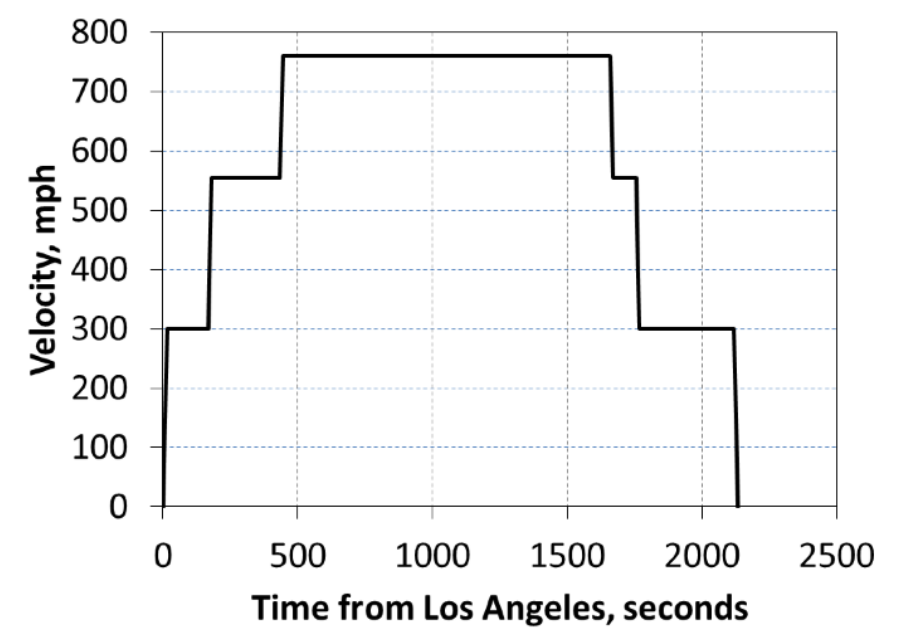
\includegraphics[scale=0.40]{figs/hyperloop.png}
\caption{Figura para el problema 1. \label{loop}}
\end{center}
\end{figure}

\begin{figure}[!h]
\begin{center}
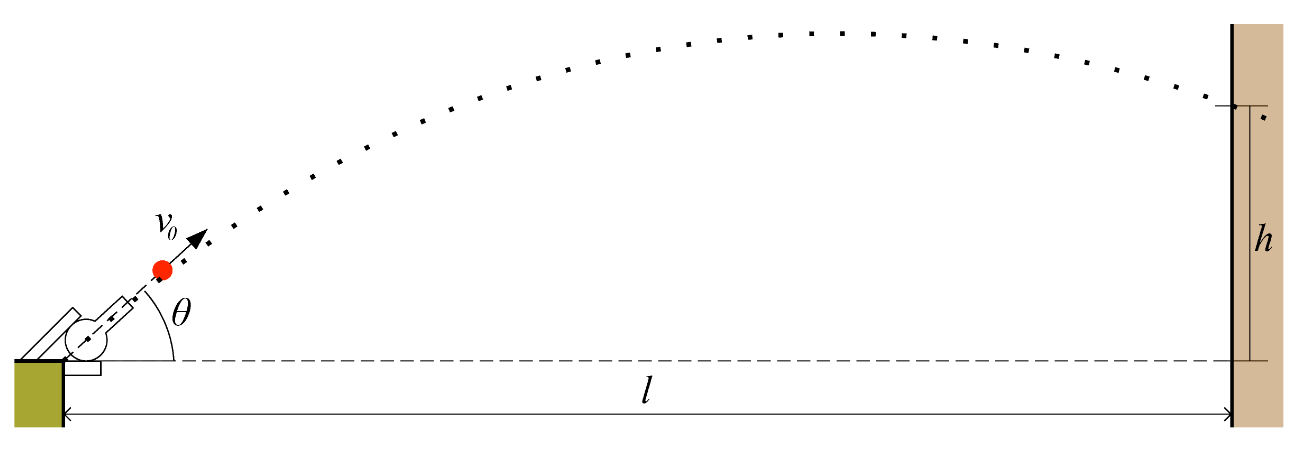
\includegraphics[scale=0.27]{figs/proyectil.png}
\caption{Figura para el problema 4. \label{proyectil}}
\end{center}
\end{figure}

{\bf NOTA}: Todas las respuestas deben tener una justificaci\'on
f\'isica y matem\'atica adecuada. Tome $g=10$ m/s$^{2}$. 100 puntos
corresponden a una calificaci\'on de 5.0.
\end{document}
